\chapter{Run-Time Support Operations}

\textsc{Perspective}: Several features of Icon's run-time system
cannot be compartmentalized as neatly as storage management but
present significant implementation problems nonetheless. These
features include type checking and conversion dereferencing and
assignment, input and output, and diagnostic facilities.

\section[12.1 Type Checking and Conversion]{12.1 Type Checking and Conversion}

Type checking is relatively straightforward in Icon. If only one type
is of interest a test of the d-word is sufficient, as in

%-% {\ttfamily\mdseries
%-% \ \ \ if (Type(Arg1) != T\_List)}
%-% 
%-% {\ttfamily\mdseries
%-% \ \ \ \ \ \ runerr(108, \&Arg1);}
\goodbreak
\iconcode{
\>if (Type(Arg1) != T\_List)\\
\>\>runerr(108, \&Arg1);
}

It is necessary to test the entire d-word, since a qualifier may have
a length that is the same as a type code. The d-word test takes care
of this, because all descriptors that are not qualifiers have \texttt{n} flags.

If different actions are needed for different types, a separate test
is required for qualifiers, since there is no type code for
strings. The RTL runtime language's \texttt{type\_case} statement
looks like a switch, but is really performing a selection according to
type generally of the form:

%-% {\ttfamily\mdseries
%-% \ \ \ if (is:string(Arg1))\textit{\ \ /* }string \textit{*/}}
%-% 
%-% {\ttfamily\mdseries
%-% \ \ \ else switch (Type(Arg1) \{}
%-% 
%-% {\ttfamily\mdseries
%-% \ \ case T\_List:\textit{\ \ /* }list \textit{*/}}
\goodbreak
\iconcode{
\>if (is:string(Arg1))\textit{\ \ /* }string \textit{*/}\\
\>\>\>\vdots\\
\>else switch (Type(Arg1) \{\\
\>\> case T\_List:\textit{\ \ /* }list \textit{*/}\\
\>\>\>\vdots
}

The real problems lie in type conversion, not type checking. At the
source-language level, type conversion can occur explicitly, as a
result of type-conversion functions, such as \texttt{string(x)}, or it
may be implicit. Implicit type conversion occurs frequently in many
kinds of computations. For example, numeric data may be read from
files in the form of strings, converted to numbers in arithmetic
computations, and then converted to strings that are written out.
Many operations support this implicit type conversion, and they rely
on type-conversion routines.

There are four types among which mutual conversion is supported:
strings, csets, integers, and real numbers. The details of type
conversion are part of the Icon language definition (Griswold and
Griswold 1983). For example, when a cset is converted to a string, the
characters of the resulting string are in lexical order. Some
conversions are conditional and may succeed or fail, depending on the
value being converted. For example, a real number can be converted to
an integer only if its value is in the range of a C long. The
conversions are illustrated in the following diagram, where dashed
lines indicate conversions that are conditional:


%--%\ \  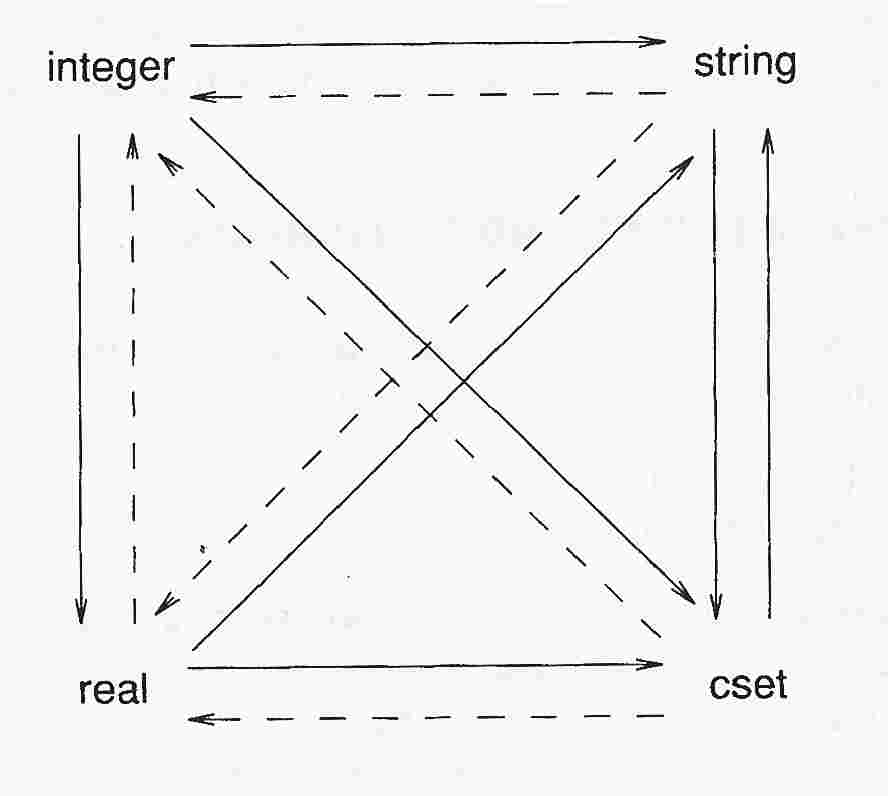
\includegraphics[width=2.9925in,height=2.6575in]{ib-img/ib-img105.jpg} 
% N.B. Can't have shorter dashed diagonal lines because LaTeX can't draw them
\begin{picture}(200,200)(-100,0)
\put(0,0){\makebox(0,0){\texttt{real}}}
\put(0,200){\makebox(0,0){\texttt{integer}}}
\put(200,0){\makebox(0,0){\texttt{cset}}}
\put(200,200){\makebox(0,0){\texttt{string}}}
\thicklines
\multiput(-4,-4)(0,200){2}{
\begin{picture}(0,0)
\put(30,10){\vector(1,0){150}}
\multiput(178,-3)(-24,0){6}{\line(-1,0){12}}\put(35,-3){\vector(-1,0){10}}
\end{picture}
}
\put(-5,170){\vector(0,-1){150}}
\multiput(10,20)(0,24){6}{\line(0,1){12}}\put(10,166){\vector(0,1){10}}
\put(190,170){\vector(0,-1){150}}
\put(205,20){\vector(0,1){150}}
\put(30,14){\vector(1,1){150}}
\multiput(30,35)(16,16){9}{\line(1,1){10}}\put(25,30){\vector(-1,-1){10}}
\multiput(170,20)(-16,16){9}{\line(-1,1){10}}\put(25,165){\vector(-1,1){10}}
\put(30,180){\vector(1,-1){150}}
\end{picture}

Thus, of the twelve conversions, five are conditional.

Some kinds of conversions are ``natural'' and occur frequently in
typical programs. Examples are string-to-integer conversion and
integer-to-string conversion. Other conversions, such as
cset-to-integer, are unlikely to occur in the normal course of
computation. To reduce the number of conversion routines required,
these unlikely conversions are done in two steps. For example, the
conversion of a cset to an integer is done by first converting the
cset to a string and then converting the string to an integer. The
direct conversions are

%--%\ \  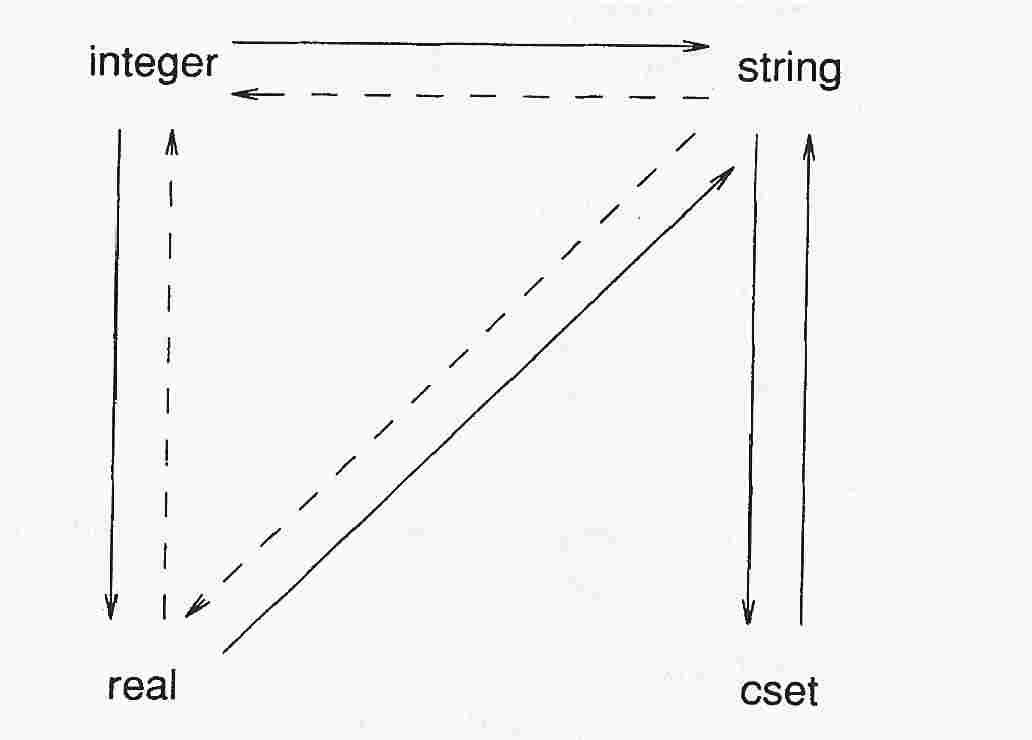
\includegraphics[width=3.5272in,height=2.4717in]{ib-img/ib-img106.jpg} 
% N.B. Can't have shorter dashed diagonal lines because LaTeX can't draw them
\begin{picture}(200,210)(-100,-10)
\put(0,0){\makebox(0,0){\texttt{real}}}
\put(0,200){\makebox(0,0){\texttt{integer}}}
\put(200,0){\makebox(0,0){\texttt{cset}}}
\put(200,200){\makebox(0,0){\texttt{string}}}
\thicklines
\put(30,206){\vector(1,0){150}}
\multiput(178,193)(-24,0){6}{\line(-1,0){12}}\put(35,193){\vector(-1,0){10}}
\put(-5,170){\vector(0,-1){150}}
\multiput(10,20)(0,24){6}{\line(0,1){12}}\put(10,166){\vector(0,1){10}}
\put(190,170){\vector(0,-1){150}}
\put(205,20){\vector(0,1){150}}
\put(30,14){\vector(1,1){150}}
\multiput(30,35)(16,16){9}{\line(1,1){10}}\put(25,30){\vector(-1,-1){10}}
\end{picture}

Conversions are done by calling routines that convert values to
expected types. These routines are

\begin{tabular}{l@{\hspace{1cm}}l}
\texttt{cnv\_cset} & convert to \texttt{cset}\\
\texttt{cnv\_int} & convert to \texttt{integer}\\
\texttt{cnv\_real} & convert to \texttt{real}\\
\texttt{cnv\_str} & convert to \texttt{string}\\
\end{tabular}

\noindent
Since these routines may be called with any type of value, all of them
are conditional. For example, it is not possible to convert a list to
a string. These routines return the value \texttt{CvtFail} to indicate
the failure of a conversion. If conversion is successful, they return
a value indicating the type of conversion.

Numerical computation introduces complications in addition to the
types integer and real, since there is the concept of a numeric
``type'' that includes both integers and real numbers. This is
represented explicitly by the Icon type-conversion function
\texttt{numeric(x)}, which converts \texttt{x} to either integer or
real, depending on the value of \texttt{x}. Its implementation
illustrates RTL's extensions to the C language for type conversions.
Rtt can generate special-case functions for each call to
\texttt{numeric(x)}, based on what it knows about the type information
at that call site, and skip the checks and conversions where they are
not necessary.

%-% {\ttfamily\mdseries
%-% function\{0,1\} numeric(n)}
%-% 
%-% {\ttfamily\mdseries
%-% \ \ \ if cnv:(exact)integer(n) then \{}
%-% 
%-% {\ttfamily\mdseries
%-% \ \ \ \ \ \ abstract \{ return integer \}}
%-% 
%-% {\ttfamily\mdseries
%-% \ \ \ \ \ \ inline \ \ \{ return n; \}}
%-% 
%-% {\ttfamily\mdseries
%-% \ \ \ \ \ \ \}}
%-% 
%-% {\ttfamily\mdseries
%-% \ \ \ else if cnv:real(n) then \{}
%-% 
%-% {\ttfamily\mdseries
%-% \ \ \ \ \ \ abstract \{ return real \}}
%-% 
%-% {\ttfamily\mdseries
%-% \ \ \ \ \ \ inline \ \ \{ return n; \}}
%-% 
%-% {\ttfamily\mdseries
%-% \ \ \ \ \ \ \}}
%-% 
%-% {\ttfamily\mdseries
%-% \ \ \ else \{}
%-% 
%-% {\ttfamily\mdseries
%-% \ \ \ \ \ \ abstract \{ return empty\_type \}}
%-% 
%-% {\ttfamily\mdseries
%-% \ \ \ \ \ \ inline \ \ \{ fail; \}}
%-% 
%-% {\ttfamily\mdseries
%-% \ \ \ \ \ \ \}}
%-% 
%-% {\ttfamily\mdseries
%-% end}
\goodbreak
\iconcode{
function\{0,1\} numeric(n)\\
\>if cnv:(exact)integer(n) then \{\\
\>\>abstract \{ return integer \}\\
\>\>inline \ \ \{ return n; \}\\
\>\>\}\\
\>else if cnv:real(n) then \{\\
\>\>abstract \{ return real \}\\
\>\>inline \ \ \{ return n; \}\\
\>\>\}\\
\>else \{\\
\>\>abstract \{ return empty\_type \}\\
\>\>inline \ \ \{ fail; \}\\
\>\>\}\\
end
}

Numeric conversion also occurs implicitly in polymorphic operations such as

{\ttfamily\mdseries
\ \ \ n+m}

\noindent which performs integer or real arithmetic, depending on the
types of \texttt{n} and \texttt{m}. The RTL language was given an
\texttt{arith\_case} construct specifically to handle this issue. The
general form of the arithmetic operators looks like:


%-% \ \ \ operator\{1\} icon\_op func\_name(x, y)
%-% 
%-% \ \ \ \ \ \ declare \{
%-% 
%-% \ \ \ \ \ \ \ \ \ tended struct descrip lx, ly;
%-% 
%-% \ \  C\_integer irslt;
%-% 
%-% \ \ \ \ \ \ \ \ \ \}
%-% 
%-% \ \ \ \ \ arith\_case (x, y) of \{
%-% 
%-% \ \ \ \ \ \ \ \ \ C\_integer: \{
%-% 
%-% \ \ \ \ \ \ \ \ \ \ \ \ abstract \{ return integer \}
%-% 
%-% \ \ \ \ \ \ \ \ \ \ \ \ inline \{
%-% 
%-% \ \ \ \ \ \ \ \ \ \ \ \ \ \ \ extern int over\_flow;
%-% 
%-% \ \ \ \ \ \ \ \ \ \ \ \ \ \ \ c\_int\_op(x,y);
%-% 
%-% \ \ \ \ \ \ \ \ \ \ \ \ \ \ \ \}
%-% 
%-% \ \ \ \ \ \ \ \ \ \ \ \ \}
%-% 
%-% \ \ \ \ \ \ \ \ \ integer: \{ /* large integers only */
%-% 
%-% \ \ \ \ \ \ \ \ \ \ \ \ abstract \{ return integer \}
%-% 
%-% \ \ \ \ \ \ \ \ \ \ \ \ inline \{
%-% 
%-% \ \ \ \ \ \ \ \ \ \ \ \ \ \ \ big\_ \#\# c\_int\_op(x,y);
%-% 
%-% \ \ \ \ \ \ \ \ \ \ \ \ \ \ \ \}
%-% 
%-% \ \ \ \ \ \ \ \ \ \ \ \ \}
%-% 
%-% \ \ \ \ \ \ \ \ \ C\_double: \{
%-% 
%-% \ \ \ \ \ \ \ \ \ \ \ \ abstract \{ return real \}
%-% 
%-% \ \ \ \ \ \ \ \ \ \ \ \ inline \{
%-% 
%-% \ \ \ \ \ \ \ \ \ \ \ \ \ \ \ c\_real\_op(x, y);
%-% 
%-% \ \ \ \ \ \ \ \ \ \ \ \ \ \ \ \}
%-% 
%-% \ \ \ \ \ \ \ \ \ \ \ \ \}
%-% 
%-% \ \ \ \ \ \ \ \ \ \}
%-% 
%-% \ \ \ end
\goodbreak
\iconcode{
\>operator\{1\} icon\_op func\_name(x, y)\\
\>\>declare \{\\
\>\>\>tended struct descrip lx, ly;\\
\ \  C\_integer irslt;\\
\>\>\>\}\\
\>\ \ arith\_case (x, y) of \{\\
\>\>\>C\_integer: \{\\
\>\>\>\>abstract \{ return integer \}\\
\>\>\>\>inline \{\\
\>\>\>\>\>extern int over\_flow;\\
\>\>\>\>\>c\_int\_op(x,y);\\
\>\>\>\>\>\}\\
\>\>\>\>\}\\
\>\>\>integer: \{ /* large integers only */\\
\>\>\>\>abstract \{ return integer \}\\
\>\>\>\>inline \{\\
\>\>\>\>\>big\_\#\# c\_int\_op(x,y);\\
\>\>\>\>\>\}\\
\>\>\>\>\}\\
\>\>\>C\_double: \{\\
\>\>\>\>abstract \{ return real \}\\
\>\>\>\>inline \{\\
\>\>\>\>\>c\_real\_op(x, y);\\
\>\>\>\>\>\}\\
\>\>\>\>\}\\
\>\>\>\}\\
\>end
}

Internally, a macro \texttt{GetReal()} is used to handle the \texttt{real}
type, since some computers have restrictions on the alignment of
\texttt{double}s. Thus, \texttt{GetReal()} has different definitions depending
on the target computer. The actual conversion of a string to a numeric
value is done by \texttt{ston()}. Note that the conversion of a cset
to a numeric value occurs by way of conversion to a string.

When types are not known at compile-time, RTL constructs such as
\texttt{cnv:str(d)} are translated down to conversion routines in
cnv.r. String conversion requires a buffer to construct the string. In
a common special-case, this buffer is provided by the routine that is
requesting string conversion for temporary use, avoiding the heap
memory allocator.  This is used, for example when a value is converted
to a string in order to convert it to a number. See Sec. 4.4.4. The
code for the ``temporary string'' version of string conversion is in a
function \texttt{tmp\_str()}:

%-% {\ttfamily\mdseries
%-% static int tmp\_str(char *sbuf, dptr s, dptr d)}
%-% 
%-% {\ttfamily\mdseries
%-% \ \ \ \{}
%-% 
%-% {\ttfamily\mdseries
%-% \ \ \ type\_case *s of \{}
%-% 
%-% {\ttfamily\mdseries
%-% \ \ \ \ \ \ string:}
%-% 
%-% {\ttfamily\mdseries
%-% \ \ \ \ \ \ \ \ \ *d = *s;}
%-% 
%-% {\ttfamily\mdseries
%-% \ \ \ \ \ \ integer: \{}
%-% 
%-% {\ttfamily\mdseries
%-% \ \ \ \ \ \ \ \ \ if (Type(*s) == T\_Lrgint) \{}
%-% 
%-% {\ttfamily\mdseries
%-% \ \ \ \ \ \ \ \ \ \ \ \ word slen, dlen;}
%-% 
%-% {\ttfamily\mdseries
%-% \ \ \ \ \ \ \ \ \ \ \ \ slen = (BlkLoc(*s)-{\textgreater}bignumblk.lsd -}
%-% 
%-% {\ttfamily\mdseries
%-% \ \ \ \ \ \ \ \ \ \ \ \ \ \ \ \ \ \ \ \ BlkLoc(*s)-{\textgreater}bignumblk.msd +1);}
%-% 
%-% {\ttfamily\mdseries
%-% \ \ \ \ \ \ \ \ \ \ \ \ dlen=slen * NB * 0.3010299956639812; /* 1/log2(10) */}
%-% 
%-% {\ttfamily\mdseries
%-% \ \ \ \ \ \ \ \ \ \ \ \ bigtos(s,d);}
%-% 
%-% {\ttfamily\mdseries
%-% \ \ \ \ \ \ \ \ \ \ \ \ \}}
%-% 
%-% {\ttfamily\mdseries
%-% \ \ \ \ \ \ \ \ \ else}
%-% 
%-% {\ttfamily\mdseries
%-% \ \ \ \ \ \ \ \ \ \ \ \ itos(IntVal(*s), d, sbuf);}
%-% 
%-% {\ttfamily\mdseries
%-% \ \ \ \ \ \ \ \ \ \}}
%-% 
%-% {\ttfamily\mdseries
%-% \ \ \ \ \ \ real: \{}
%-% 
%-% {\ttfamily\mdseries
%-% \ \ \ \ \ \ \ \ \ double res;}
%-% 
%-% {\ttfamily\mdseries
%-% \ \ \ \ \ \ \ \ \ GetReal(s, res);}
%-% 
%-% {\ttfamily\mdseries
%-% \ \ \ \ \ \ \ \ \ rtos(res, d, sbuf);}
%-% 
%-% {\ttfamily\mdseries
%-% \ \ \ \ \ \ \ \ \ \}}
%-% 
%-% {\ttfamily\mdseries
%-% \ \ \ \ \ \ cset:}
%-% 
%-% {\ttfamily\mdseries
%-% \ \ \ \ \ \ \ \ \ cstos(BlkLoc(*s)-{\textgreater}cset.bits, d, sbuf);}
%-% 
%-% {\ttfamily\mdseries
%-% \ \ \ \ \ \ default:}
%-% 
%-% {\ttfamily\mdseries
%-% \ \ \ \ \ \ \ \ \ return 0;}
%-% 
%-% {\ttfamily\mdseries
%-% \ \ \ \ \ \ \}}
%-% 
%-% {\ttfamily\mdseries
%-% \ \ \ return 1;}
%-% 
%-% {\ttfamily\mdseries
%-% \ \ \ \}}
\goodbreak
\iconcode{
static int tmp\_str(char *sbuf, dptr s, dptr d)\\
\>\{\\
\>type\_case *s of \{\\
\>\>string:\\
\>\>\>*d = *s;\\
\>\>integer: \{\\
\>\>\>if (Type(*s) == T\_Lrgint) \{\\
\>\>\>\>word slen, dlen;\\
\>\>\>\>slen = (BlkLoc(*s)->bignumblk.lsd -\\
\>\>\>\>\>\>\ \ BlkLoc(*s)->bignumblk.msd +1);\\
\>\>\>\>dlen=slen * NB * 0.3010299956639812; /* 1/log2(10) */\\
\>\>\>\>bigtos(s,d);\\
\>\>\>\>\}\\
\>\>\>else\\
\>\>\>\>itos(IntVal(*s), d, sbuf);\\
\>\>\>\}\\
\>\>real: \{\\
\>\>\>double res;\\
\>\>\>GetReal(s, res);\\
\>\>\>rtos(res, d, sbuf);\\
\>\>\>\}\\
\>\>cset:\\
\>\>\>cstos(BlkLoc(*s)->cset.bits, d, sbuf);\\
\>\>default:\\
\>\>\>return 0;\\
\>\>\}\\
\>return 1;\\
\>\}
}

If a conversion is required, \texttt{itos()}, \texttt{rtos()}, or
\texttt{cstos()} does the actual work, placing its result in \texttt{sbuf} and
changing the descriptor pointed to by \texttt{d} accordingly. These routines
return a 1 if the result is a string and a 0 otherwise. The monitoring
facilities in Unicon can also report whether no conversion was needed
(\texttt{E\_Nconv}), a conversion was performed successfully
(\texttt{E\_Sconv}), or the conversion failed (\texttt{E\_Fconv}).

If a converted string is in a buffer that is local to the calling
routine, it must be copied into allocated storage, or it would be
destroyed when that routine returns. The fully general version of
\texttt{cnv\_str()} is equivalent to the following function. Because
this function is heavily called, in reality the body of
\texttt{tmp\_str()} is inlined in \texttt{cnv\_str()}.

%-% {\ttfamily\mdseries
%-% int cnv\_str(dptr s, dptr d)}
%-% 
%-% {\ttfamily\mdseries
%-% \ \ \ \{}
%-% 
%-% {\ttfamily\mdseries
%-% \ \ \ char sbuf[MaxCvtLen];}
%-% 
%-% 
%-% \bigskip
%-% 
%-% {\ttfamily\mdseries
%-% \ \ \ type\_case *s of \{}
%-% 
%-% {\ttfamily\mdseries
%-% \ \ \ \ \ \ string: \{}
%-% 
%-% {\ttfamily\mdseries
%-% \ \ \ \ \ \ \ \ \ *d = *s;}
%-% 
%-% {\ttfamily\mdseries
%-% \ \ \ \ \ \ \ \ \ return 1;}
%-% 
%-% {\ttfamily\mdseries
%-% \ \ \ \ \ \ \ \ \ \}}
%-% 
%-% {\ttfamily\mdseries
%-% \ \ \ \ \ \ default: \{}
%-% 
%-% {\ttfamily\mdseries
%-% \ \ \ \ \ \ \ \ \ if (!tmp\_str(sbuf, s, d)) return 0;}
%-% 
%-% {\ttfamily\mdseries
%-% \ \ \ \ \ \ \ \ \ \}}
%-% 
%-% {\ttfamily\mdseries
%-% \ \ \ \ \ \ \}}
%-% 
%-% {\ttfamily\mdseries
%-% \ \ \ Protect(StrLoc(*d) =}
%-% 
%-% {\ttfamily\mdseries
%-% \ \ \ \ \ \ \ \ \ \ \ \ \ \ alcstr(StrLoc(*d), StrLen(*d)), fatalerr(0,NULL));}
%-% 
%-% {\ttfamily\mdseries
%-% \ \ \ return 1;}
%-% 
%-% {\ttfamily\mdseries
%-% \ \ \ \}}
\goodbreak
\iconcode{
int cnv\_str(dptr s, dptr d)\\
\>\{\\
\>char sbuf[MaxCvtLen];\\
\\
\>type\_case *s of \{\\
\>\>string: \{\\
\>\>\>*d = *s;\\
\>\>\>return 1;\\
\>\>\>\}\\
\>\>default: \{\\
\>\>\>if (!tmp\_str(sbuf, s, d)) return 0;\\
\>\>\>\}\\
\>\>\}\\
\>Protect(StrLoc(*d) = alcstr(StrLoc(*d), StrLen(*d)), fatalerr(0,NULL));\\
\>return 1;\\
\>\}
}

\section[12.2 Dereferencing and Assignment]{12.2 Dereferencing and Assignment}

If there were no trapped variables, dereferencing and assignment would
be trivial. For example, the descriptor \texttt{d} is dereferenced by

%-% {\ttfamily\mdseries
%-% \ \ \ d = *VarLoc(d)}
\iconline{ \>d = *VarLoc(d) }

\noindent where \texttt{VarLoc} references the v-word of \texttt{d}:

%-% {\ttfamily\mdseries
%-% \ \ \ \#define VarLoc(d) ((d).vword.dptr)}
\iconline{\>\#define VarLoc(d) ((d).vword.dptr) }

The dereferencing or assignment to a trapped variable, on the other
hand, may involve a complicated computation. This computation reflects
the meaning associated with the operation on the source-language
expression that is represented in the implementation as a trapped
variable. For example, as discussed previously, in

%-% {\ttfamily\mdseries
%-% \textit{\ \ \ }x[y] := z}
\iconline{ \textit{\ \ \ }x[y] := z }

\noindent the value of \texttt{x} may be a list, a string, a table, or a
record. A subscripted list or record does not produce a trapped
variable, but the other two cases do. For a string, the variable on
the left side of the assignment is a substring trapped variable. For a
table, the variable is a table-element trapped variable. In the first
case, the assignment involves the concatenation of three strings and
the assignment of the result to \texttt{x}. In the second case, it involves
looking for \texttt{y} in the table. If there is a table element for \texttt{y}, its
assigned value is changed to the value of \texttt{z}.  Otherwise, the
table-element trapped-variable block is converted to a table-element
block with the assigned value, and the block is inserted in the
appropriate chain.

\subsection[12.2.1 Dereferencing]{12.2.1 Dereferencing}

Dereferencing of other trapped variables involves computations of
comparable complexity. Dereferencing is done in the interpreter loop
for arguments of operators for which variables are not needed. For
example, in

%-% {\ttfamily\mdseries
%-% \ \ \ n+m}
\iconline{ \>n+m }

\noindent the identifiers \texttt{n} and \texttt{m} are dereferenced before the function
for addition is called (See Sec. 8.3.1). On the other hand, in

{\ttfamily\mdseries
\ \ \ s[i]}

\noindent the identifier \texttt{i} is dereferenced, but \texttt{s} is not, since the
subscripting routine needs the variable as well as its value.

The function invocation routine also dereferences variables before a
function is called. Note that there is no function that requires an
argument that is a variable. Suspension and return from procedures
also dereference local identifiers and arguments. Dereferencing occurs
in a number of other places. For example, the function that handles
subscripting must dereference the subscripted variable to determine
what kind of result to produce.

The dereferencing routine begins as follows:

%-% {\ttfamily\mdseries
%-% void deref(s, d)}
%-% 
%-% {\ttfamily\mdseries
%-% dptr s, d;}
%-% 
%-% {\ttfamily\mdseries
%-% \ \ \ \{}
%-% 
%-% {\ttfamily\mdseries
%-% \ \ \ /*}
%-% 
%-% {\ttfamily\mdseries
%-% \ \ \ \ * no allocation is done, so nothing need be tended.}
%-% 
%-% {\ttfamily\mdseries
%-% \ \ \ \ */}
%-% 
%-% {\ttfamily\mdseries
%-% \ \ \ register union block *bp, **ep;}
%-% 
%-% {\ttfamily\mdseries
%-% \ \ \ struct descrip v;}
%-% 
%-% {\ttfamily\mdseries
%-% \ \ \ int res;}
%-% 
%-% 
%-% \bigskip
%-% 
%-% {\ttfamily\mdseries
%-% \ \ \ if (!is:variable(*s)) \{}
%-% 
%-% {\ttfamily\mdseries
%-% \ \ \ \ \ \ *d = *s;}
%-% 
%-% {\ttfamily\mdseries
%-% \ \ \ \ \ \ \}}
\goodbreak
\iconcode{
void deref(s, d)\\
dptr s, d;\\
\>\{\\
\>/*\\
\>\ * no allocation is done, so nothing need be tended.\\
\>\ */\\
\>register union block *bp, **ep;\\
\>struct descrip v;\\
\>int res;\\
\\
\>if (!is:variable(*s)) \{\\
\>\>*d = *s;\\
\>\>\}
}


\noindent
If \texttt{s} does not point to a variable descriptor, the remaining code is skipped.

If \texttt{s} points to a variable that is not a trapped variable,
dereferencing is simple:

%-% {\ttfamily\mdseries
%-% \ \ \ \ \ \ \ \ \ /*}
%-% 
%-% {\ttfamily\mdseries
%-% \ \ \ \ \ \ \ \ \ \ * An ordinary variable is being dereferenced.}
%-% 
%-% {\ttfamily\mdseries
%-% \ \ \ \ \ \ \ \ \ \ */}
%-% 
%-% {\ttfamily\mdseries
%-% \ \ \ \ \ \ \ \ \ *d = *(dptr)((word *)VarLoc(*s) + Offset(*s));}
\goodbreak
\iconcode{
\>\>\>/*\\
\>\>\>\ * An ordinary variable is being dereferenced.\\
\>\>\>\ */\\
\>\>\>*d = *(dptr)((word *)VarLoc(*s) + Offset(*s));
}

Otherwise, there are three types of trapped variables with a switch on the type:

%-% {\ttfamily\mdseries
%-% \ \ \ type\_case *s of \{}
%-% 
%-% {\ttfamily\mdseries
%-% \ \ \ \ \ \ tvsubs: \{}
%-% 
%-% {\ttfamily\mdseries
%-% \ \ \ \ \ \ \ \ \ /*}
%-% 
%-% {\ttfamily\mdseries
%-% \ \ \ \ \ \ \ \ \ \ * A substring trapped variable is being dereferenced.}
%-% 
%-% {\ttfamily\mdseries
%-% \ \ \ \ \ \ \ \ \ \ * \ Point bp to the trapped variable block and v to}
%-% 
%-% {\ttfamily\mdseries
%-% \ \ \ \ \ \ \ \ \ \ * \ the string.}
%-% 
%-% {\ttfamily\mdseries
%-% \ \ \ \ \ \ \ \ \ \ */}
%-% 
%-% {\ttfamily\mdseries
%-% \ \ \ \ \ \ \ \ \ bp = BlkLoc(*s);}
%-% 
%-% {\ttfamily\mdseries
%-% \ \ \ \ \ \ \ \ \ deref(\&bp-{\textgreater}tvsubs.ssvar, \&v);}
%-% 
%-% {\ttfamily\mdseries
%-% \ \ \ \ \ \ \ \ \ if (!is:string(v))}
%-% 
%-% {\ttfamily\mdseries
%-% \ \ \ \ \ \ \ \ \ \ \ \ fatalerr(103, \&v);}
%-% 
%-% {\ttfamily\mdseries
%-% \ \ \ \ \ \ \ \ \ if (bp-{\textgreater}tvsubs.sspos + bp-{\textgreater}tvsubs.sslen - 1 {\textgreater} StrLen(v))}
%-% 
%-% {\ttfamily\mdseries
%-% \ \ \ \ \ \ \ \ \ \ \ \ fatalerr(205, NULL);}
%-% 
%-% {\ttfamily\mdseries
%-% \ \ \ \ \ \ \ \ \ /*}
%-% 
%-% {\ttfamily\mdseries
%-% \ \ \ \ \ \ \ \ \ \ * Make a descriptor for the substring by getting the}
%-% 
%-% {\ttfamily\mdseries
%-% \ \ \ \ \ \ \ \ \ \ * \ length and pointing into the string.}
%-% 
%-% {\ttfamily\mdseries
%-% \ \ \ \ \ \ \ \ \ \ */}
%-% 
%-% {\ttfamily\mdseries
%-% \ \ \ \ \ \ \ \ \ StrLen(*d) = bp-{\textgreater}tvsubs.sslen;}
%-% 
%-% {\ttfamily\mdseries
%-% \ \ \ \ \ \ \ \ \ StrLoc(*d) = StrLoc(v) + bp-{\textgreater}tvsubs.sspos - 1;}
%-% 
%-% {\ttfamily\mdseries
%-% \ \ \ \ \ \ \ \ \}}
%-% 
%-% 
%-% \bigskip
%-% 
%-% {\ttfamily\mdseries
%-% \ \ \ \ \ \ tvtbl: \{}
%-% 
%-% {\ttfamily\mdseries
%-% \ \ \ \ \ \ \ \ \ /*}
%-% 
%-% {\ttfamily\mdseries
%-% \ \ \ \ \ \ \ \ \ \ * Look up the element in the table.}
%-% 
%-% {\ttfamily\mdseries
%-% \ \ \ \ \ \ \ \ \ \ */}
%-% 
%-% {\ttfamily\mdseries
%-% \ \ \ \ \ \ \ \ \ bp = BlkLoc(*s);}
%-% 
%-% {\ttfamily\mdseries
%-% \ \ \ \ \ \ \ \ \ ep = memb(bp-{\textgreater}tvtbl.clink,\&bp-{\textgreater}tvtbl.tref,}
%-% 
%-% {\ttfamily\mdseries
%-% \ \ \ \ \ \ \ \ \ \ \ \ \ \ \ \ \ \ \ bp-{\textgreater}tvtbl.hashnum,\&res);}
%-% 
%-% {\ttfamily\mdseries
%-% \ \ \ \ \ \ \ \ \ if (res == 1)}
%-% 
%-% {\ttfamily\mdseries
%-% \ \ \ \ \ \ \ \ \ \ \ \ *d = (*ep)-{\textgreater}telem.tval;\ \ /* found; use value */}
%-% 
%-% {\ttfamily\mdseries
%-% \ \ \ \ \ \ \ \ \ else}
%-% 
%-% {\ttfamily\mdseries
%-% \ \ \ \ \ \ \ \ \ \ \ \ *d = bp-{\textgreater}tvtbl.clink-{\textgreater}table.defvalue;/*use default */}
%-% 
%-% {\ttfamily\mdseries
%-% \ \ \ \ \ \ \ \ \ \}}
\goodbreak
\iconcode{
\>type\_case *s of \{\\
\>\>tvsubs: \{\\
\>\>\>/*\\
\>\>\>\ * A substring trapped variable is being dereferenced.\\
\>\>\>\ * \ Point bp to the trapped variable block and v to\\
\>\>\>\ * \ the string.\\
\>\>\>\ */\\
\>\>\>bp = BlkLoc(*s);\\
\>\>\>deref(\&bp->tvsubs.ssvar, \&v);\\
\>\>\>if (!is:string(v))\\
\>\>\>\>fatalerr(103, \&v);\\
\>\>\>if (bp->tvsubs.sspos + bp->tvsubs.sslen - 1 > StrLen(v))\\
\>\>\>\>fatalerr(205, NULL);\\
\>\>\>/*\\
\>\>\>\ * Make a descriptor for the substring by getting the\\
\>\>\>\ * \ length and pointing into the string.\\
\>\>\>\ */\\
\>\>\>StrLen(*d) = bp->tvsubs.sslen;\\
\>\>\>StrLoc(*d) = StrLoc(v) + bp->tvsubs.sspos - 1;\\
\>\>\ \ \}\\
\\
\>\>tvtbl: \{\\
\>\>\>/*\\
\>\>\>\ * Look up the element in the table.\\
\>\>\>\ */\\
\>\>\>bp = BlkLoc(*s);\\
\>\>\>ep = memb(bp->tvtbl.clink,\&bp->tvtbl.tref,\\
\>\>\>\>\>\>\ bp->tvtbl.hashnum,\&res);\\
\>\>\>if (res == 1)\\
\>\>\>\>*d = (*ep)->telem.tval;\ \ /* found; use value */\\
\>\>\>else\\
\>\>\>\>*d = bp->tvtbl.clink->table.defvalue;/*use default */\\
\>\>\>\}
}

A table-element trapped variable may point to a table-element
trapped-variable block or to a table-element block. The second
situation occurs if two table-element trapped variables point to the
same table-element trapped-variable block and assignment to one of the
variables converts the table-element trapped-variable block to a
table-element block before the second variable is processed. See
Sec. 7.2. In this case, the value of the trapped variable is in the
table-element block. On the other hand, if the trapped variable points
to a table-element trapped-variable block, it is necessary to look up
the subscripting value in the table, since an assignment for it may
have been made between the time the trapped variable was created and
the time it was dereferenced. If it is in the table, the corresponding
assigned value is returned. If it is not in the table, the default
assigned value is returned.

The last case, keyword trapped variables, is almost the same as for
simple variables. These variables impose special semantics on
assignment, but not on dereferencing.

%-% {\ttfamily\mdseries
%-% \ \ \ \ \ \ kywdint:}
%-% 
%-% {\ttfamily\mdseries
%-% \ \ \ \ \ \ kywdpos:}
%-% 
%-% {\ttfamily\mdseries
%-% \ \ \ \ \ \ kywdsubj:}
%-% 
%-% {\ttfamily\mdseries
%-% \ \ \ \ \ \ kywdevent:}
%-% 
%-% {\ttfamily\mdseries
%-% \ \ \ \ \ \ kywdwin:}
%-% 
%-% {\ttfamily\mdseries
%-% \ \ \ \ \ \ kywdstr:}
%-% 
%-% 
%-% \ \ \ \ \ \ \ \ \ *d = *VarLoc(*s);
\goodbreak
\iconcode{
\>\>kywdint:\\
\>\>kywdpos:\\
\>\>kywdsubj:\\
\>\>kywdevent:\\
\>\>kywdwin:\\
\>\>kywdstr:\\
\>\>\>*d = *VarLoc(*s);
}

\subsection[12.2.2 Assignment]{12.2.2 Assignment}

The values of global identifiers are established initially as a
byproduct of reading the icode file into the icode region. When
procedures are called, the values of arguments and local identifiers
are on the interpreter stack. These operations associate values with
variables, but assignment, unlike dereferencing, is explicit in the
source program.


The macro \texttt{GeneralAsgn()} is used to perform all such
operations. For example, the function for

%-% {\ttfamily\mdseries
%-% \ \ \ x := y}
\iconline{ \>x := y }

is

%-% {\ttfamily\mdseries
%-% operator\{0,1\} := asgn(underef x, y)}
%-% 
%-% {\ttfamily\mdseries
%-% \ \ \ if !is:variable(x) then}
%-% 
%-% {\ttfamily\mdseries
%-% \ \ \ \ \ \ runerr(111, x)}
%-% 
%-% {\ttfamily\mdseries
%-% \ \ \ abstract \{}
%-% 
%-% {\ttfamily\mdseries
%-% \ \ \ \ \ \ return type(x)}
%-% 
%-% {\ttfamily\mdseries
%-% \ \ \ \ \ \ \}}
%-% 
%-% {\ttfamily\mdseries
%-% \ \ \ GeneralAsgn(x, y)}
%-% 
%-% {\ttfamily\mdseries
%-% \ \ \ inline \{}
%-% 
%-% {\ttfamily\mdseries
%-% \ \ \ \ \ \ /*}
%-% 
%-% {\ttfamily\mdseries
%-% \ \ \ \ \ \ \ * The returned result is the variable to which assignment }
%-% 
%-% {\ttfamily\mdseries
%-% \ \ \ \ \ \ \ * \ is being made.}
%-% 
%-% {\ttfamily\mdseries
%-% \ \ \ \ \ \ \ */}
%-% 
%-% {\ttfamily\mdseries
%-% \ \ \ \ \ \ return x;}
%-% 
%-% {\ttfamily\mdseries
%-% \ \ \ \ \ \ \}}
%-% 
%-% {\ttfamily\mdseries
%-% end}
\goodbreak
\iconcode{
operator\{0,1\} := asgn(underef x, y)\\
\>if !is:variable(x) then\\
\>\>runerr(111, x)\\
\>abstract \{\\
\>\>return type(x)\\
\>\>\}\\
\>GeneralAsgn(x, y)\\
\>inline \{\\
\>\>/*\\
\>\>\ * The returned result is the variable to which assignment \\
\>\>\ * \ is being made.\\
\>\>\ */\\
\>\>return x;\\
\>\>\}\\
end
}

Note that assignment may fail. This can occur as the result of an
out-of-range assignment to \texttt{\&pos} and is indicated by an RTL
\texttt{fail} statement from within \texttt{GeneralAsgn()}.

Like dereferencing, assignment is trivial for variables that are not
trapped. The macro \texttt{GeneralAsgn()} begins as follows:

%-% {\ttfamily\mdseries
%-% \#begdef GeneralAsgn(x, y)}
%-% 
%-% \bigskip
%-% 
%-% {\ttfamily\mdseries
%-% \ \ \ type\_case x of \{}
\goodbreak
\iconcode{
\#begdef GeneralAsgn(x, y)\\
\>type\_case x of \{
}

As for dereferencing, there are three types of trapped variables to be
considered. Assignment to a substring trapped variable is rather
complicated and deferred to a function \texttt{subs\_asgn()}:

%-% {\ttfamily\mdseries
%-% \ \ \ \ \ \ tvsubs: \{}
%-% 
%-% {\ttfamily\mdseries
%-% \ \ \ \ \ \ \ \ abstract \{}
%-% 
%-% {\ttfamily\mdseries
%-% \ \ \ \ \ \ \ \ \ \ \ store[store[type(x).str\_var]] = string}
%-% 
%-% {\ttfamily\mdseries
%-% \ \ \ \ \ \ \ \ \ \ \ \}}
%-% 
%-% {\ttfamily\mdseries
%-% \ \ \ \ \ \ \ \ inline \{}
%-% 
%-% {\ttfamily\mdseries
%-% \ \ \ \ \ \ \ \ \ \ \ if (subs\_asgn(\&x, (const dptr)\&y) == Error)}
%-% 
%-% {\ttfamily\mdseries
%-% \ \ \ \ \ \ \ \ \ \ \ \ \ \ runerr(0);}
%-% 
%-% {\ttfamily\mdseries
%-% \ \ \ \ \ \ \ \ \ \ \ \}}
%-% 
%-% {\ttfamily\mdseries
%-% \ \ \ \ \ \ \ \ \}}
\goodbreak
\iconcode{
\>\>tvsubs: \{\\
\>\>\ \ abstract \{\\
\>\>\>\ \ store[store[type(x).str\_var]] = string\\
\>\>\>\ \ \}\\
\>\>\ \ inline \{\\
\>\>\>\ \ if (subs\_asgn(\&x, (const dptr)\&y) == Error)\\
\>\>\>\>\ \ runerr(0);\\
\>\>\>\ \ \}\\
\>\>\ \ \}
}

The function \texttt{subs\_asgn()}:

%-% {\ttfamily\mdseries
%-% int subs\_asgn(dptr dest, const dptr src)}
%-% 
%-% {\ttfamily\mdseries
%-% \ \ \ \{}
%-% 
%-% {\ttfamily\mdseries
%-% \ \ \ tended struct descrip deststr, srcstr, rsltstr;}
%-% 
%-% {\ttfamily\mdseries
%-% \ \ \ tended struct b\_tvsubs *tvsub;}
%-% 
%-% 
%-% \bigskip
%-% 
%-% {\ttfamily\mdseries
%-% \ \ \ char *s, *s2;}
%-% 
%-% {\ttfamily\mdseries
%-% \ \ \ word i, len;}
%-% 
%-% {\ttfamily\mdseries
%-% \ \ \ word prelen;/* length of portion of string before substring */}
%-% 
%-% {\ttfamily\mdseries
%-% \ \ \ word poststrt, postlen; /* start and length of portion of}
%-% 
%-% {\ttfamily\mdseries
%-% \ \ \ \ \ \ \ \ \ \ \ \ \ \ \ \ \ \ \ \ \ \ \ \ \ \ \ \ \ \ string following substring */}
%-% 
%-% {\ttfamily\mdseries
%-% \ \ \ if (!cnv:tmp\_string(*src, srcstr))}
%-% 
%-% {\ttfamily\mdseries
%-% \ \ \ \ \ \ ReturnErrVal(103, *src, Error);}
%-% 
%-% {\ttfamily\mdseries
%-% \ \ \ /*}
%-% 
%-% {\ttfamily\mdseries
%-% \ \ \ \ * Be sure that the variable in the trapped variable points}
%-% 
%-% {\ttfamily\mdseries
%-% \ \ \ \ * \ to a string and that the string is big enough to contain}
%-% 
%-% {\ttfamily\mdseries
%-% \ \ \ \ * \ the substring.}
%-% 
%-% {\ttfamily\mdseries
%-% \ \ \ \ */}
%-% 
%-% {\ttfamily\mdseries
%-% \ \ \ tvsub = (struct b\_tvsubs *)BlkLoc(*dest);}
%-% 
%-% {\ttfamily\mdseries
%-% \ \ \ deref(\&tvsub-{\textgreater}ssvar, \&deststr);}
%-% 
%-% {\ttfamily\mdseries
%-% \ \ \ if (!is:string(deststr))}
%-% 
%-% {\ttfamily\mdseries
%-% \ \ \ \ \ \ ReturnErrVal(103, deststr, Error);}
%-% 
%-% {\ttfamily\mdseries
%-% \ \ \ prelen = tvsub-{\textgreater}sspos - 1;}
%-% 
%-% {\ttfamily\mdseries
%-% \ \ \ poststrt = prelen + tvsub-{\textgreater}sslen;}
%-% 
%-% {\ttfamily\mdseries
%-% \ \ \ if (poststrt {\textgreater} StrLen(deststr))}
%-% 
%-% {\ttfamily\mdseries
%-% \ \ \ \ \ \ ReturnErrNum(205, Error);}
%-% 
%-% 
%-% \bigskip
%-% 
%-% {\ttfamily\mdseries
%-% \ \ \ /*}
%-% 
%-% {\ttfamily\mdseries
%-% \ \ \ \ * Form the result string.}
%-% 
%-% {\ttfamily\mdseries
%-% \ \ \ \ * \ Start by allocating space for the entire result.}
%-% 
%-% {\ttfamily\mdseries
%-% \ \ \ \ */}
%-% 
%-% {\ttfamily\mdseries
%-% \ \ \ len = prelen + StrLen(srcstr) + StrLen(deststr) - poststrt;}
%-% 
%-% {\ttfamily\mdseries
%-% \ \ \ Protect(s = alcstr(NULL, len), return Error);}
%-% 
%-% {\ttfamily\mdseries
%-% \ \ \ StrLoc(rsltstr) = s;}
%-% 
%-% {\ttfamily\mdseries
%-% \ \ \ StrLen(rsltstr) = len;}
%-% 
%-% {\ttfamily\mdseries
%-% \ \ \ /*}
%-% 
%-% {\ttfamily\mdseries
%-% \ \ \ \ * First, copy the portion of the substring string to}
%-% 
%-% {\ttfamily\mdseries
%-% \ \ \ \ * \ the left of the substring into the string space.}
%-% 
%-% {\ttfamily\mdseries
%-% \ \ \ \ */}
%-% 
%-% {\ttfamily\mdseries
%-% \ \ \ s2 = StrLoc(deststr);}
%-% 
%-% {\ttfamily\mdseries
%-% \ \ \ for (i = 0; i {\textless} prelen; i++)}
%-% 
%-% {\ttfamily\mdseries
%-% \ \ \ \ \ \ *s++ = *s2++;}
%-% 
%-% {\ttfamily\mdseries
%-% \ \ \ /*}
%-% 
%-% {\ttfamily\mdseries
%-% \ \ \ \ * Copy the string to be assigned into the string space,}
%-% 
%-% {\ttfamily\mdseries
%-% \ \ \ \ * \ effectively concatenating it.}
%-% 
%-% {\ttfamily\mdseries
%-% \ \ \ \ */}
%-% 
%-% {\ttfamily\mdseries
%-% \ \ \ s2 = StrLoc(srcstr);}
%-% 
%-% {\ttfamily\mdseries
%-% \ \ \ for (i = 0; i {\textless} StrLen(srcstr); i++)}
%-% 
%-% {\ttfamily\mdseries
%-% \ \ \ \ \ \ *s++ = *s2++;}
%-% 
%-% {\ttfamily\mdseries
%-% \ \ \ /*}
%-% 
%-% {\ttfamily\mdseries
%-% \ \ \ \ * Copy the portion of the substring to the right of the}
%-% 
%-% {\ttfamily\mdseries
%-% \ \ \ \ * \ substring into the string space, completing the result.}
%-% 
%-% {\ttfamily\mdseries
%-% \ \ \ \ */}
%-% 
%-% {\ttfamily\mdseries
%-% \ \ \ s2 = StrLoc(deststr) + poststrt;}
%-% 
%-% {\ttfamily\mdseries
%-% \ \ \ postlen = StrLen(deststr) - poststrt;}
%-% 
%-% {\ttfamily\mdseries
%-% \ \ \ for (i = 0; i {\textless} postlen; i++)}
%-% 
%-% {\ttfamily\mdseries
%-% \ \ \ \ \ \ *s++ = *s2++;}
%-% 
%-% 
%-% \bigskip
%-% 
%-% {\ttfamily\mdseries
%-% \ \ \ /*}
%-% 
%-% {\ttfamily\mdseries
%-% \ \ \ \ * Perform the assignment and update the trapped variable.}
%-% 
%-% {\ttfamily\mdseries
%-% \ \ \ \ */}
%-% 
%-% {\ttfamily\mdseries
%-% \ \ \ type\_case tvsub-{\textgreater}ssvar of \{}
%-% 
%-% {\ttfamily\mdseries
%-% \ \ \ \ \ \ kywdevent: \{}
%-% 
%-% {\ttfamily\mdseries
%-% \ \ \ \ \ \ \ \ \ *VarLoc(tvsub-{\textgreater}ssvar) = rsltstr;}
%-% 
%-% {\ttfamily\mdseries
%-% \ \ \ \ \ \ \ \ \ \}}
%-% 
%-% {\ttfamily\mdseries
%-% \ \ \ \ \ \ kywdstr: \{}
%-% 
%-% {\ttfamily\mdseries
%-% \ \ \ \ \ \ \ \ \ *VarLoc(tvsub-{\textgreater}ssvar) = rsltstr;}
%-% 
%-% {\ttfamily\mdseries
%-% \ \ \ \ \ \ \ \ \ \}}
%-% 
%-% {\ttfamily\mdseries
%-% \ \ \ \ \ \ kywdsubj: \{}
%-% 
%-% {\ttfamily\mdseries
%-% \ \ \ \ \ \ \ \ \ *VarLoc(tvsub-{\textgreater}ssvar) = rsltstr;}
%-% 
%-% {\ttfamily\mdseries
%-% \ \ \ \ \ \ \ \ \ k\_pos = 1;}
%-% 
%-% {\ttfamily\mdseries
%-% \ \ \ \ \ \ \ \ \ \}}
%-% 
%-% {\ttfamily\mdseries
%-% \ \ \ \ \ \ tvtbl: \{}
%-% 
%-% {\ttfamily\mdseries
%-% \ \ \ \ \ \ \ \ \ if (tvtbl\_asgn(\&tvsub-{\textgreater}ssvar, (const dptr)\&rsltstr) ==}
%-% 
%-% {\ttfamily\mdseries
%-% \ \ \ \ \ \ \ \ \ \ \ \ \ \ \ Error)}
%-% 
%-% {\ttfamily\mdseries
%-% \ \ \ \ \ \ \ \ \ \ \ \ return Error;}
%-% 
%-% {\ttfamily\mdseries
%-% \ \ \ \ \ \ \ \ \ \}}
%-% 
%-% {\ttfamily\mdseries
%-% \ \ \ \ \ \ default: \{}
%-% 
%-% {\ttfamily\mdseries
%-% \ \ \ \ \ \ \ \ \ Asgn(tvsub-{\textgreater}ssvar, rsltstr);}
%-% 
%-% {\ttfamily\mdseries
%-% \ \ \ \ \ \ \ \ \ \}}
%-% 
%-% {\ttfamily\mdseries
%-% \ \ \ \ \ \ \}}
%-% 
%-% {\ttfamily\mdseries
%-% \ \ \ tvsub-{\textgreater}sslen = StrLen(srcstr);}
%-% 
%-% {\ttfamily\mdseries
%-% \ \ \ return Succeeded;}
%-% 
%-% {\ttfamily\mdseries
%-% \ \ \ \}}
\goodbreak
\iconcode{
int subs\_asgn(dptr dest, const dptr src)\\
\>\{\\
\>tended struct descrip deststr, srcstr, rsltstr;\\
\>tended struct b\_tvsubs *tvsub;\\
\\
\>char *s, *s2;\\
\>word i, len;\\
\>word prelen;/* length of portion of string before substring */\\
\>word poststrt, postlen; /* start and length of portion of\\
\>\>\>\>\>\>\>\>\>\>string following substring */\\
\>if (!cnv:tmp\_string(*src, srcstr))\\
\>\>ReturnErrVal(103, *src, Error);\\
\>/*\\
\>\ * Be sure that the variable in the trapped variable points\\
\>\ * \ to a string and that the string is big enough to contain\\
\>\ * \ the substring.\\
\>\ */\\
\>tvsub = (struct b\_tvsubs *)BlkLoc(*dest);\\
\>deref(\&tvsub->ssvar, \&deststr);\\
\>if (!is:string(deststr))\\
\>\>ReturnErrVal(103, deststr, Error);\\
\>prelen = tvsub->sspos - 1;\\
\>poststrt = prelen + tvsub->sslen;\\
\>if (poststrt > StrLen(deststr))\\
\>\>ReturnErrNum(205, Error);\\
\\
\>/*\\
\>\ * Form the result string.\\
\>\ * \ Start by allocating space for the entire result.\\
\>\ */\\
\>len = prelen + StrLen(srcstr) + StrLen(deststr) - poststrt;\\
\>Protect(s = alcstr(NULL, len), return Error);\\
\>StrLoc(rsltstr) = s;\\
\>StrLen(rsltstr) = len;\\
\>/*\\
\>\ * First, copy the portion of the substring string to\\
\>\ * \ the left of the substring into the string space.\\
\>\ */\\
\>s2 = StrLoc(deststr);\\
\>for (i = 0; i < prelen; i++)\\
\>\>*s++ = *s2++;\\
\>/*\\
\>\ * Copy the string to be assigned into the string space,\\
\>\ * \ effectively concatenating it.\\
\>\ */\\
\>s2 = StrLoc(srcstr);\\
\>for (i = 0; i < StrLen(srcstr); i++)\\
\>\>*s++ = *s2++;\\
\>/*\\
\>\ * Copy the portion of the substring to the right of the\\
\>\ * \ substring into the string space, completing the result.\\
\>\ */\\
\>s2 = StrLoc(deststr) + poststrt;\\
\>postlen = StrLen(deststr) - poststrt;\\
\>for (i = 0; i < postlen; i++)\\
\>\>*s++ = *s2++;\\
\\
\>/*\\
\>\ * Perform the assignment and update the trapped variable.\\
\>\ */\\
\>type\_case tvsub->ssvar of \{\\
\>\>kywdevent: \{\\
\>\>\>*VarLoc(tvsub->ssvar) = rsltstr;\\
\>\>\>\}\\
\>\>kywdstr: \{\\
\>\>\>*VarLoc(tvsub->ssvar) = rsltstr;\\
\>\>\>\}\\
\>\>kywdsubj: \{\\
\>\>\>*VarLoc(tvsub->ssvar) = rsltstr;\\
\>\>\>k\_pos = 1;\\
\>\>\>\}\\
\>\>tvtbl: \{\\
\>\>\>if (tvtbl\_asgn(\&tvsub->ssvar, (const dptr)\&rsltstr) == Error)\\
\>\>\>\>return Error;\\
\>\>\>\}\\
\>\>default: \{\\
\>\>\>Asgn(tvsub->ssvar, rsltstr);\\
\>\>\>\}\\
\>\>\}\\
\>tvsub->sslen = StrLen(srcstr);\\
\>return Succeeded;\\
\>\}\\
}

Table-element trapped variables are once again deferred in
\texttt{GeneralAsgn()} to call to a function, \texttt{tvtbl\_asgn()}:

%-% {\ttfamily\mdseries
%-% \ \ \ \ \ \ tvtbl: \{}
%-% 
%-% {\ttfamily\mdseries
%-% \ \ \ \ \ \ \ \ abstract \{}
%-% 
%-% {\ttfamily\mdseries
%-% \ \ \ \ \ \ \ \ \ \ \ store[store[type(x).trpd\_tbl].tbl\_val] = type(y)}
%-% 
%-% {\ttfamily\mdseries
%-% \ \ \ \ \ \ \ \ \ \ \ \}}
%-% 
%-% {\ttfamily\mdseries
%-% \ \ \ \ \ \ \ \ inline \{}
%-% 
%-% {\ttfamily\mdseries
%-% \ \ \ \ \ \ \ \ \ \ \ if (tvtbl\_asgn(\&x, (const dptr)\&y) == Error)}
%-% 
%-% {\ttfamily\mdseries
%-% \ \ \ \ \ \ \ \ \ \ \ \ \ \ runerr(0);}
%-% 
%-% {\ttfamily\mdseries
%-% \ \ \ \ \ \ \ \ \ \ \ \}}
%-% 
%-% {\ttfamily\mdseries
%-% \ \ \ \ \ \ \ \ \ \}}
\goodbreak
\iconcode{
\>\>tvtbl: \{\\
\>\>\ \ abstract \{\\
\>\>\>\ \ store[store[type(x).trpd\_tbl].tbl\_val] = type(y)\\
\>\>\>\ \ \}\\
\>\>\ \ inline \{\\
\>\>\>\ \ if (tvtbl\_asgn(\&x, (const dptr)\&y) == Error)\\
\>\>\>\>\ \ runerr(0);\\
\>\>\>\ \ \}\\
\>\>\>\}
}

Table-element trapped variables have the same possibilities for
assignment as for dereferencing. The processing is more complicated,
since it may be necessary to convert a table-element trapped-variable
block into a table-element block and link it into a chain. Parameters
cannot be tended, so their information must be preserved in tended
variables before anything is allocated.

%-% {\ttfamily\mdseries
%-% int tvtbl\_asgn(dptr dest, const dptr src)}
%-% 
%-% {\ttfamily\mdseries
%-% \ \ \ \{}
%-% 
%-% {\ttfamily\mdseries
%-% \ \ \ tended struct b\_tvtbl *bp;}
%-% 
%-% {\ttfamily\mdseries
%-% \ \ \ tended struct descrip tval;}
%-% 
%-% {\ttfamily\mdseries
%-% \ \ \ struct b\_telem *te;}
%-% 
%-% {\ttfamily\mdseries
%-% \ \ \ union block **slot;}
%-% 
%-% {\ttfamily\mdseries
%-% \ \ \ struct b\_table *tp;}
%-% 
%-% {\ttfamily\mdseries
%-% \ \ \ int res;}
%-% 
%-% \bigskip
%-% 
%-% {\ttfamily\mdseries
%-% \ \ \ /*}
%-% 
%-% {\ttfamily\mdseries
%-% \ \ \ \ * Allocate table element now (even if we may not need it)}
%-% 
%-% {\ttfamily\mdseries
%-% \ \ \ \ * because slot cannot be tended. Parameters have to be}
%-% 
%-% {\ttfamily\mdseries
%-% \ \ \ \ * preserved in tended variables first.}
%-% 
%-% {\ttfamily\mdseries
%-% \ \ \ \ */}
%-% 
%-% {\ttfamily\mdseries
%-% \ \ \ bp = (struct b\_tvtbl *) BlkLoc(*dest);}
%-% 
%-% {\ttfamily\mdseries
%-% \ \ \ tval = *src;}
%-% 
%-% {\ttfamily\mdseries
%-% \ \ \ Protect(te = alctelem(), return Error);}
%-% 
%-% 
%-% \bigskip
%-% 
%-% {\ttfamily\mdseries
%-% \ \ \ /*}
%-% 
%-% {\ttfamily\mdseries
%-% \ \ \ \ * First see if reference is in the table; if it is, just }
%-% 
%-% {\ttfamily\mdseries
%-% \ \ \ \ * \ update the value. \ Otherwise, allocate a new table entry.}
%-% 
%-% {\ttfamily\mdseries
%-% \ \ \ \ */}
%-% 
%-% {\ttfamily\mdseries
%-% \ \ \ slot = memb(bp-{\textgreater}clink, \&bp-{\textgreater}tref, bp-{\textgreater}hashnum, \&res);}
%-% 
%-% 
%-% \bigskip
%-% 
%-% {\ttfamily\mdseries
%-% \ \ \ if (res == 1) \{}
%-% 
%-% {\ttfamily\mdseries
%-% \ \ \ \ \ \ /*}
%-% 
%-% {\ttfamily\mdseries
%-% \ \ \ \ \ \ \ * Do not need new te, just update existing entry.}
%-% 
%-% {\ttfamily\mdseries
%-% \ \ \ \ \ \ \ */}
%-% 
%-% {\ttfamily\mdseries
%-% \ \ \ \ \ \ deallocate((union block *) te);}
%-% 
%-% {\ttfamily\mdseries
%-% \ \ \ \ \ \ (*slot)-{\textgreater}telem.tval = tval;}
%-% 
%-% {\ttfamily\mdseries
%-% \ \ \ \ \ \ \}}
%-% 
%-% {\ttfamily\mdseries
%-% \ \ \ else \{}
%-% 
%-% {\ttfamily\mdseries
%-% \ \ \ \ \ \ /*}
%-% 
%-% {\ttfamily\mdseries
%-% \ \ \ \ \ \ \ * Link te into table, fill in entry.}
%-% 
%-% {\ttfamily\mdseries
%-% \ \ \ \ \ \ \ */}
%-% 
%-% {\ttfamily\mdseries
%-% \ \ \ \ \ \ tp = (struct b\_table *) bp-{\textgreater}clink;}
%-% 
%-% {\ttfamily\mdseries
%-% \ \ \ \ \ \ tp-{\textgreater}size++;}
%-% 
%-% 
%-% \bigskip
%-% 
%-% {\ttfamily\mdseries
%-% \ \ \ \ \ \ te-{\textgreater}clink = *slot;}
%-% 
%-% {\ttfamily\mdseries
%-% \ \ \ \ \ \ *slot = (union block *) te;}
%-% 
%-% 
%-% \bigskip
%-% 
%-% {\ttfamily\mdseries
%-% \ \ \ \ \ \ te-{\textgreater}hashnum = bp-{\textgreater}hashnum;}
%-% 
%-% {\ttfamily\mdseries
%-% \ \ \ \ \ \ te-{\textgreater}tref = bp-{\textgreater}tref;}
%-% 
%-% {\ttfamily\mdseries
%-% \ \ \ \ \ \ te-{\textgreater}tval = tval;}
%-% 
%-% 
%-% \bigskip
%-% 
%-% {\ttfamily\mdseries
%-% \ \ \ \ \ \ if (TooCrowded(tp))\ \ /* grow hash table if now too full */}
%-% 
%-% {\ttfamily\mdseries
%-% \ \ \ \ \ \ \ \ \ hgrow((union block *)tp);}
%-% 
%-% {\ttfamily\mdseries
%-% \ \ \ \ \ \ \}}
%-% 
%-% {\ttfamily\mdseries
%-% \ \ \ return Succeeded;}
%-% 
%-% {\ttfamily\mdseries
%-% \ \ \ \}}
\goodbreak
\iconcode{
int tvtbl\_asgn(dptr dest, const dptr src)\\
\{\\
\>tended struct b\_tvtbl *bp;\\
\>tended struct descrip tval;\\
\>struct b\_telem *te;\\
\>union block **slot;\\
\>struct b\_table *tp;\\
\>int res;\\
\\
\>/*\\
\>\ * Allocate table element now (even if we may not need it)\\
\>\ * because slot cannot be tended. Parameters have to be\\
\>\ * preserved in tended variables first.\\
\>\ */\\
\>bp = (struct b\_tvtbl *) BlkLoc(*dest);\\
\>tval = *src;\\
\>Protect(te = alctelem(), return Error);\\
\\
\>/*\\
\>\ * First see if reference is in the table; if it is, just \\
\>\ * \ update the value. \ Otherwise, allocate a new table entry.\\
\>\ */\\
\>slot = memb(bp->clink, \&bp->tref, bp->hashnum, \&res);\\
\\
\>if (res == 1) \{\\
\>\>/*\\
\>\>\ * Do not need new te, just update existing entry.\\
\>\>\ */\\
\>\>deallocate((union block *) te);\\
\>\>(*slot)->telem.tval = tval;\\
\>\>\}\\
\>else \{\\
\>\>/*\\
\>\>\ * Link te into table, fill in entry.\\
\>\>\ */\\
\>\>tp = (struct b\_table *) bp->clink;\\
\>\>tp->size++;\\
\\
\>\>te->clink = *slot;\\
\>\>*slot = (union block *) te;\\
\\
\>\>te->hashnum = bp->hashnum;\\
\>\>te->tref = bp->tref;\\
\>\>te->tval = tval;\\
\\
\>\>if (TooCrowded(tp))\ \ /* grow hash table if now too full */\\
\>\>\>hgrow((union block *)tp);\\
\>\>\}\\
\>return Succeeded;\\
\}
}

In the case of a keyword trapped variable, the semantic requirements
of the keyword are expressed in the usual mixture of RTL and C, except
that type information is guaranteed not to change. The code for
\texttt{\&subject} is typical:

%-% {\ttfamily\mdseries
%-% \ \ \ \ \ \ kywdsubj: \{}
%-% 
%-% {\ttfamily\mdseries
%-% \ \ \ \ \ \ \ \ \ /*}
%-% 
%-% {\ttfamily\mdseries
%-% \ \ \ \ \ \ \ \ \ \ * No side effect in the type realm = no abstract clause}
%-% 
%-% {\ttfamily\mdseries
%-% \ \ \ \ \ \ \ \ \ \ * \ \&subject is still a string and \&pos is still an int.}
%-% 
%-% {\ttfamily\mdseries
%-% \ \ \ \ \ \ \ \ \ \ */}
%-% 
%-% {\ttfamily\mdseries
%-% \ \ \ \ \ \ \ \ \ if !cnv:string(y, *VarLoc(x)) then}
%-% 
%-% {\ttfamily\mdseries
%-% \ \ \ \ \ \ \ \ \ \ \ \ runerr(103, y);}
%-% 
%-% {\ttfamily\mdseries
%-% \ \ \ \ \ \ \ \ \ inline \{}
%-% 
%-% {\ttfamily\mdseries
%-% \ \ \ \ \ \ \ \ \ \ \ \ k\_pos = 1;}
%-% 
%-% {\ttfamily\mdseries
%-% \ \ \ \ \ \ \ \ \ \ \ \ \}}
%-% 
%-% {\ttfamily\mdseries
%-% \ \ \ \ \ \ \ \ \ \}}
\goodbreak
\iconcode{
\>\>kywdsubj: \{\\
\>\>\>/*\\
\>\>\>\ * No side effect in the type realm = no abstract clause\\
\>\>\>\ * \ \&subject is still a string and \&pos is still an int.\\
\>\>\>\ */\\
\>\>\>if !cnv:string(y, *VarLoc(x)) then\\
\>\>\>\>runerr(103, y);\\
\>\>\>inline \{\\
\>\>\>\>k\_pos = 1;\\
\>\>\>\>\}\\
\>\>\>\}
}

\section[12.3 Input and Output]{12.3 Input and Output}

Icon supports only sequential file access. The run-time system uses C
library routines to perform input and output, so the main
implementation issues are those that relate to interfacing these
routines.

\subsection[12.3.1 Files]{12.3.1 Files}

A value of type file in Icon points to a block that contains the usual
title word, a \texttt{FILE *} reference to the file, a status word,
and the string name of the file. The file status values include


\begin{tabular}{l@{\hspace{1cm}}l}
0 & closed\\
1 & open for reading\\
2 & open for writing\\
4 & open to create\\
8 & open to append\\
16 & open as a pipe\\
\end{tabular}

\noindent These decimal numbers correspond to bits in the status word.

For example, the value of \texttt{\&input} is


%--%\ \  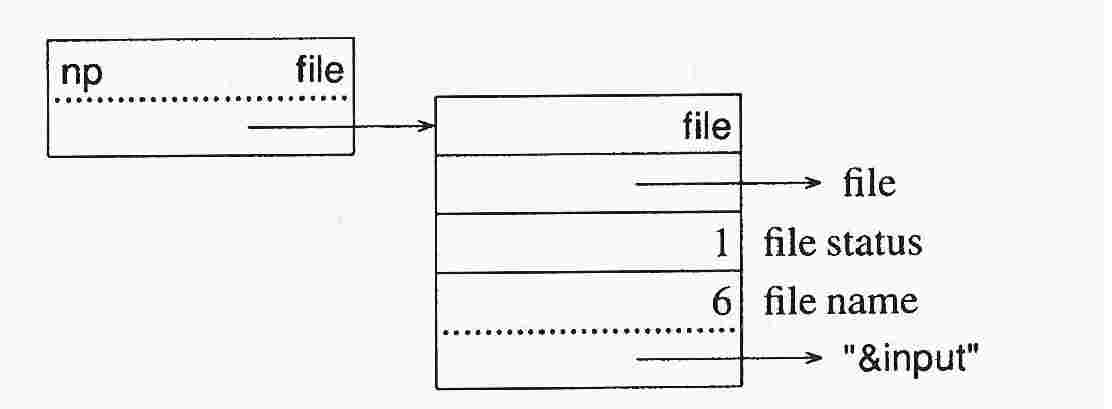
\includegraphics[width=3.7402in,height=1.3661in]{ib-img/ib-img107.jpg} 
\begin{picture}(300,100)
\put(120,0){\dvboxptr{6}{}{40}{\texttt{"\&input"}}}
\put(120,0){\trboxlabel{file name}}
\put(120,32){\wordbox{1}{}}
\put(120,32){\brboxlabel{file status}}
\put(120,48){\blkboxptr{file}{40}{file}}
\put(0,64){\dvboxptr{file}{np}{40}{}}
\end{picture}

\noindent while the value of \texttt{\&output} is


%--%\ \  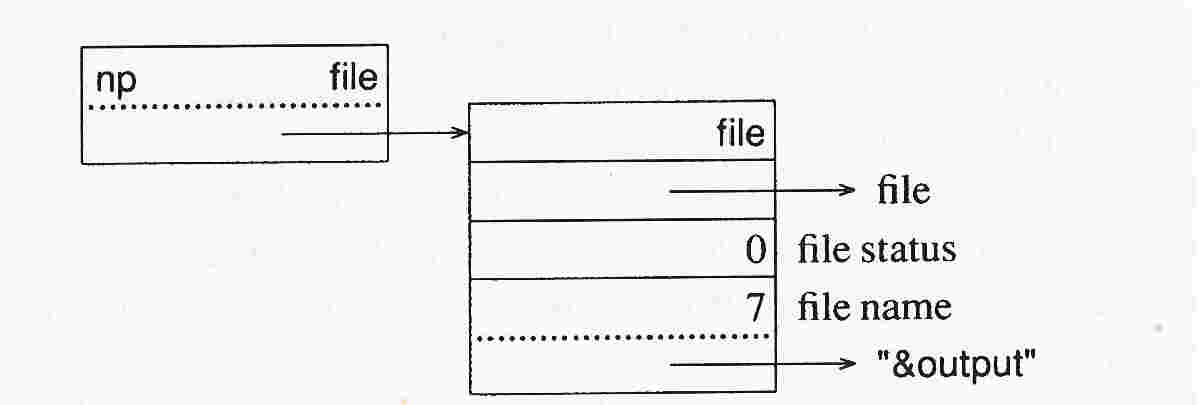
\includegraphics[width=4.0602in,height=1.352in]{ib-img/ib-img108.jpg} 
\begin{picture}(300,100)
\put(120,0){\dvboxptr{7}{}{40}{\texttt{"\&output"}}}
\put(120,0){\trboxlabel{file name}}
\put(120,32){\wordbox{2}{}}
\put(120,32){\brboxlabel{file status}}
\put(120,48){\blkboxptr{file}{40}{file}}
\put(0,64){\dvboxptr{file}{np}{40}{}}
\end{picture}

Another example is

%-% {\ttfamily\mdseries
%-% \ \ \ out := open({\textquotedbl}log{\textquotedbl}, {\textquotedbl}a{\textquotedbl})}
\iconline{ \>out := open("log", "a") }

\noindent for which the value of \texttt{out} is


%--%\ \  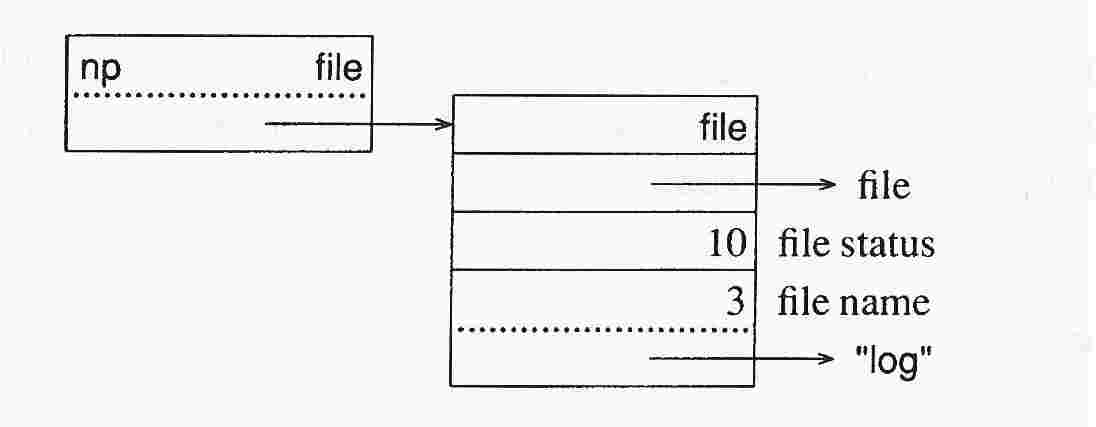
\includegraphics[width=3.7402in,height=1.4252in]{ib-img/ib-img109.jpg} 
\begin{picture}(300,100)
\put(120,0){\dvboxptr{3}{}{40}{\texttt{"log"}}}
\put(120,0){\trboxlabel{file name}}
\put(120,32){\wordbox{10}{}}
\put(120,32){\brboxlabel{file status}}
\put(120,48){\blkboxptr{file}{40}{file}}
\put(0,64){\dvboxptr{file}{np}{40}{}}
\end{picture}

Note that the file status is 10, corresponding to being open for
writing and appending.

Closing a file, as in

%-% {\ttfamily\mdseries
%-% \ \ \ close(out)}
\iconline{ \>close(out) }

\noindent merely changes its file status:

%--%\ \  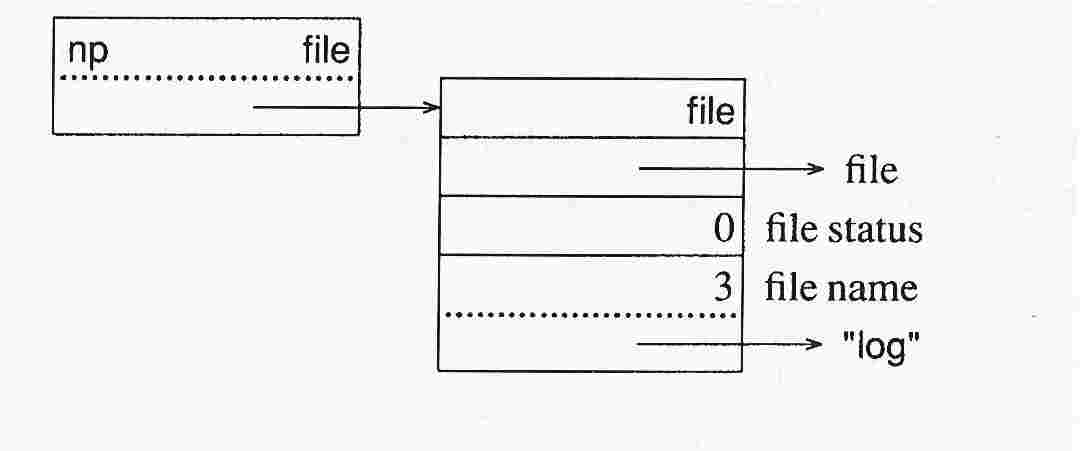
\includegraphics[width=3.6335in,height=1.5063in]{ib-img/ib-img110.jpg} 
\begin{picture}(300,100)
\put(120,0){\dvboxptr{3}{}{40}{\texttt{"log"}}}
\put(120,0){\trboxlabel{file name}}
\put(120,32){\wordbox{0}{}}
\put(120,32){\brboxlabel{file status}}
\put(120,48){\blkboxptr{file}{40}{file}}
\put(0,64){\dvboxptr{file}{np}{40}{}}
\end{picture}

\subsection[12.3.2 Reading and Writing Data]{12.3.2 Reading and Writing Data}

The function \texttt{read(f)} reads a line from the file
\texttt{f}. In UNIX, a line is just a string of characters up to a
newline character. There is no limit on the length of a line and the
length of a line cannot be determined before it is read. On the other
hand, there must be a place to store the line.

Characters are read into a buffer until a newline character is
encountered or the buffer size (by default 512) is reached. A
predictive need request is then made to assure that there is enough
space in the allocated string region for the string, and the string is
copied from the buffer into the string region. This is repeated as
needed.

The function \texttt{reads(f,i)} reads \texttt{i} characters from the
file \texttt{f}. These characters may include newline
characters. There is no limit on \texttt{i} other than available
memory. A predictive need request can be made to assure that there is
enough space in the allocated string region. Characters are then read
directly into the allocated string region without the use of an
intervening buffer.

When strings are written, they are written directly from the allocated
string region. There is no need to perform any allocation or to use an
intermediate buffer.

Several strings can be concatenated on a file by

%-% {\ttfamily\mdseries
%-% \ \ \ write(s1 , s2, ..., sn)}
\iconline{ \>write(s1 , s2, ..., sn) }

This avoids the internal allocation and concatenation that is required for

%-% {\ttfamily\mdseries
%-% \ \ \ write(s1 {\textbar}{\textbar} s2 {\textbar}{\textbar} ...{\textbar}{\textbar} sn)}
\iconline{ \>write(s1 || s2 || ...|| sn) }

\section[12.4 Diagnostic Facilities]{12.4 Diagnostic Facilities}

Icon's diagnostic facilities consist of

\liststyleLxvii
\begin{itemize}

\item The function \texttt{image(x)}, which produces a string
representation of the value of \texttt{x}.

\item The function \texttt{display(f, i)}, which writes the names and
values of identifiers in at most \texttt{i} levels of procedure call
to the file \texttt{f}.

\item Tracing of procedure calls, returns, resumptions, and suspensions.

\item Run-time error termination messages.

\end{itemize}

Procedure tracing is done in the virtual machine instructions \texttt{invoke},
\texttt{pret}, \texttt{pfail}, and \texttt{psusp}. If the value of \texttt{\&trace} is nonzero,
it is decremented and an appropriate trace message is written to
standard error output.  See Sec. 2.1.12 for an example.

The function \texttt{display(f,i)} must locate the names and values of
local identifiers and arguments. The names are in the procedure block
for the current procedure, which is pointed to by the zeroth argument
of the current procedure call. The values are on the interpreter stack
as described in Sec. 10.3.3.

Run-time termination messages are produced by the C routine
\texttt{runerr(n,dp)}, where \texttt{dp} is a pointer to the
descriptor for the offending value. The value NULL is used for
\texttt{dp} in cases where there is no offending value to print.

In all of these diagnostic situations, string representations of
values are needed. The string representation for the
{\textquotedbl}scalar{\textquotedbl} types string, cset, integer, and
real is similar to what it is in the text of a source-language
program. Long strings and csets are truncated to provide output that
is easy to read. Other types present a variety of problems. For
procedures, the type and procedure name are given.

A list, on the other hand, may be arbitrarily large and may contain
values of any type, even lists. While the name may suffice for a
procedure, often more information about a list is needed. As a
compromise between information content and readability, only the first
three and last three elements of a long list are included in its
string representation.  Since lists and other non-scalar types may be
elements of lists, their representation as elements of a list is more
restricted, with only the type and size being shown.

Since trace, display, and error output are written to files, the
string representations can be written as they are determined, without
regard for how long they are. The function \texttt{image(x)}, on the
other hand, returns a string value, and space must be allocated for
it. A more limited form of string representation is used for
non-scalar values, since the space needed might otherwise be very
large.

\bigskip

\noindent\textbf{EXERCISES}

\noindent {\bf 12.1} It is possible to conceive of meaningful ways to convert
\textit{any} type of data in Icon to any other. For example, a
procedure might be converted to a string that consists of the
procedure declaration. How would such a general conversion feature
affect the way that types are converted in the run-time system?

\noindent {\bf 12.2} On computers with 16-bit words, Icon has two
representations for integers internally (see Sec. 4.1.3). Describe how
this complicates type conversion.

\noindent {\bf 12.3} How would the addition of a new numeric type,
such as complex numbers, affect type conversion?

\noindent {\bf 12.4} How big would \texttt{MaxCvtLen} be if Icon had 512
different characters?  128? 64?

\noindent {\bf 12.5} List all the source-language operations that
perform assignment.

\noindent {\bf 12.6} Assuming that \texttt{x}, \texttt{y}, \texttt{z},
and \texttt{w} all have string values, diagram the structures that are
produced in the course of evaluating the following expressions:
\iconcode{
x[y] := z\\
z := x[y]\\
x[y] := z[w]\\
x[y][z] := w
}
Repeat this exercise for the case where all the identifiers have tables as values.

\noindent {\bf 12.7} Give an expression in which a table-element
trapped variable points to a table-element block rather than to a
table-element trapped-variable block.

\noindent {\bf 12.8} Give an expression in which a table-element
trapped variable points to a table-element trapped-variable block, but
where there is a table-element block in the table with the same entry
value.

\noindent {\bf 12.9} 
Why are tended descriptors needed in assignment but not in dereferencing?

\noindent {\bf 12.10} Show an expression in which, at the end of the case for
assignment to a substring trapped variable, the variable to which the
assignment is to be made is a trapped variable. Can such a trapped
variable be of any of the three types?

\noindent {\bf 12.11} Why is the string produced by \texttt{read(f)}
not read directly into the allocated string region?

\noindent {\bf 12.12} Are there any circumstances in which
\texttt{write(x1, x2, ..., xn)} requires the allocation of storage?

\noindent {\bf 12.13} Identify all the portions of blocks for
source-language values that are necessary only for diagnostic
output. How significant is the amount of space involved?

\noindent {\bf 12.14} The use of trapped variables for keywords that
require special processing for assignment suggests that a similar
technique might be used for substring and table-element trapped
variables. Evaluate this possibility.
